% LM122A Pablo Rodrigo Sanches
\documentclass[12pt,a4paper]{article} \usepackage[utf8]{inputenc}
\usepackage[onehalfspacing]{setspace}
\usepackage[lmargin=3cm,tmargin=3cm,rmargin=2cm,bmargin=2cm]{geometry}
\usepackage[brazil]{babel} \usepackage[T1]{fontenc} \usepackage{graphicx}
\usepackage{indentfirst} \usepackage{comment} \usepackage{enumerate}
\usepackage{hyperref} \usepackage{tabularx} \usepackage{subfig}
\usepackage[normalem]{ulem}
\hypersetup{ colorlinks=true, linkcolor=blue, filecolor=magenta, urlcolor=cyan,
}

% numeracao header
\pagestyle{headings}

% quebra de pagina por secao

\begin{document}

\begin{titlepage}
	\begin{center}
		\textbf{UNIVERSIDADE DE RIBEIRÃO PRETO} \\
		CIÊNCIAS EXATAS \\
		Iteração Humano Computador

			\vspace{1.5cm}

			\textbf{Prof. Fernando Marco Perez Campos} \vspace{3.5cm}

			\textbf{GUSTAVO CASTRO NUNES  765954} \\
			\textbf{GABRIEL DA SILVA ARAUJO 834856} \\
			\textbf{MURILO IJANC’ 834125} \\
			\textbf{JORDANA C. DE PAIVA 832994} \\
			\textbf{GUILHERME REIS 833206} \\
			\textbf{EDSON DA SILVA LEITE JUNIOR 833156} \\
			\textbf{WERNER MENDONÇA DE MORAIS 767306} \\

			\vspace{3.5cm}

			\textbf{ATIVIDADE PARCIAL}

			\vfill

			\vspace{0.8cm}

			
\includegraphics[width=0.2\textwidth]{unaerp}

			\textbf{RIBEIRÃO PRETO} \\
			\textbf{2020}
	\end{center}
\end{titlepage}


\thispagestyle{empty}

\tableofcontents

\newpage

\thispagestyle{empty} \listoffigures \thispagestyle{empty} \newpage

\pagenumbering{arabic}

% secao 1
\section{Introdução} Nesse projeto iremos apresentar um controle tecnológico
baseado na Domótica, que basicamente é a implantação de tecnologia nas
residências ou comércios a fim de encontrar soluções que deem resposta à
necessidade do homem de querer realizar o mínimo esforço nas atividades diárias
e rotineiras além do controle também promover segurança. Consideramos também a
importância da utilização dessa tecnologia de forma fácil ao usuário comum,
pensando na usabilidade e no cumprimento das heurísticas de Nielsen.

\section{Elicitação de requisitos} A técnica de elicitação de requisitos
utilizada pelo grupo foi de Brainstorm, pois é a que melhor se adequou para o
desenvolvimento do grupo devido a “chuva” de idéias boas e ruins, que foram
sendo utilizadas ou descartadas para chegarmos ao objetivo pré-determinado,  de
um controle acessível e funcional.

\section{Documentação} O controle remoto seria ativado por botões mais sensor
de voz. Os botões teriam escrito abaixo deles qual aparelho eles ativariam e
teriam uma letra em braille, que permitiria que o controle fosse utilizado por
pessoas cegas. O sensor de voz também ajudaria as pessoas cegas e serviria como
um conforto extra para os outros usuários. Com essas opções o controle consegue
atender os tipos de deficiências mais comuns, como cegos, surdos, mudos e
paraplégicos. Tetraplégicos poderiam utilizar o controle através do sensor de
voz.  O controle utilizaria tecnologia wifi e bluetooth para se comunicar com
os aparelhos na asa e realizar suas funções, por exemplo:

\begin{itemize}
	\item abrir/fechar janelas ou cortinas (acoplando-se um motor a elas)
	\item trancar/destrancar portas
	\item ligar/desligar ar
		condicionados/ventiladores
	\item controlar a temperatura do ar condicionado
	\item ligar/desligar alarmes
	\item ligar/desligar luzes
	\item controlar a intensidade da luz
	\item ligar/desligar aparelhos eletrônicos (televisores,
videogames, rádios)
\item mudar o volume e canais da televisão
\end{itemize}

\section{Layout}
\begin{figure}[htb!]
	\centering
	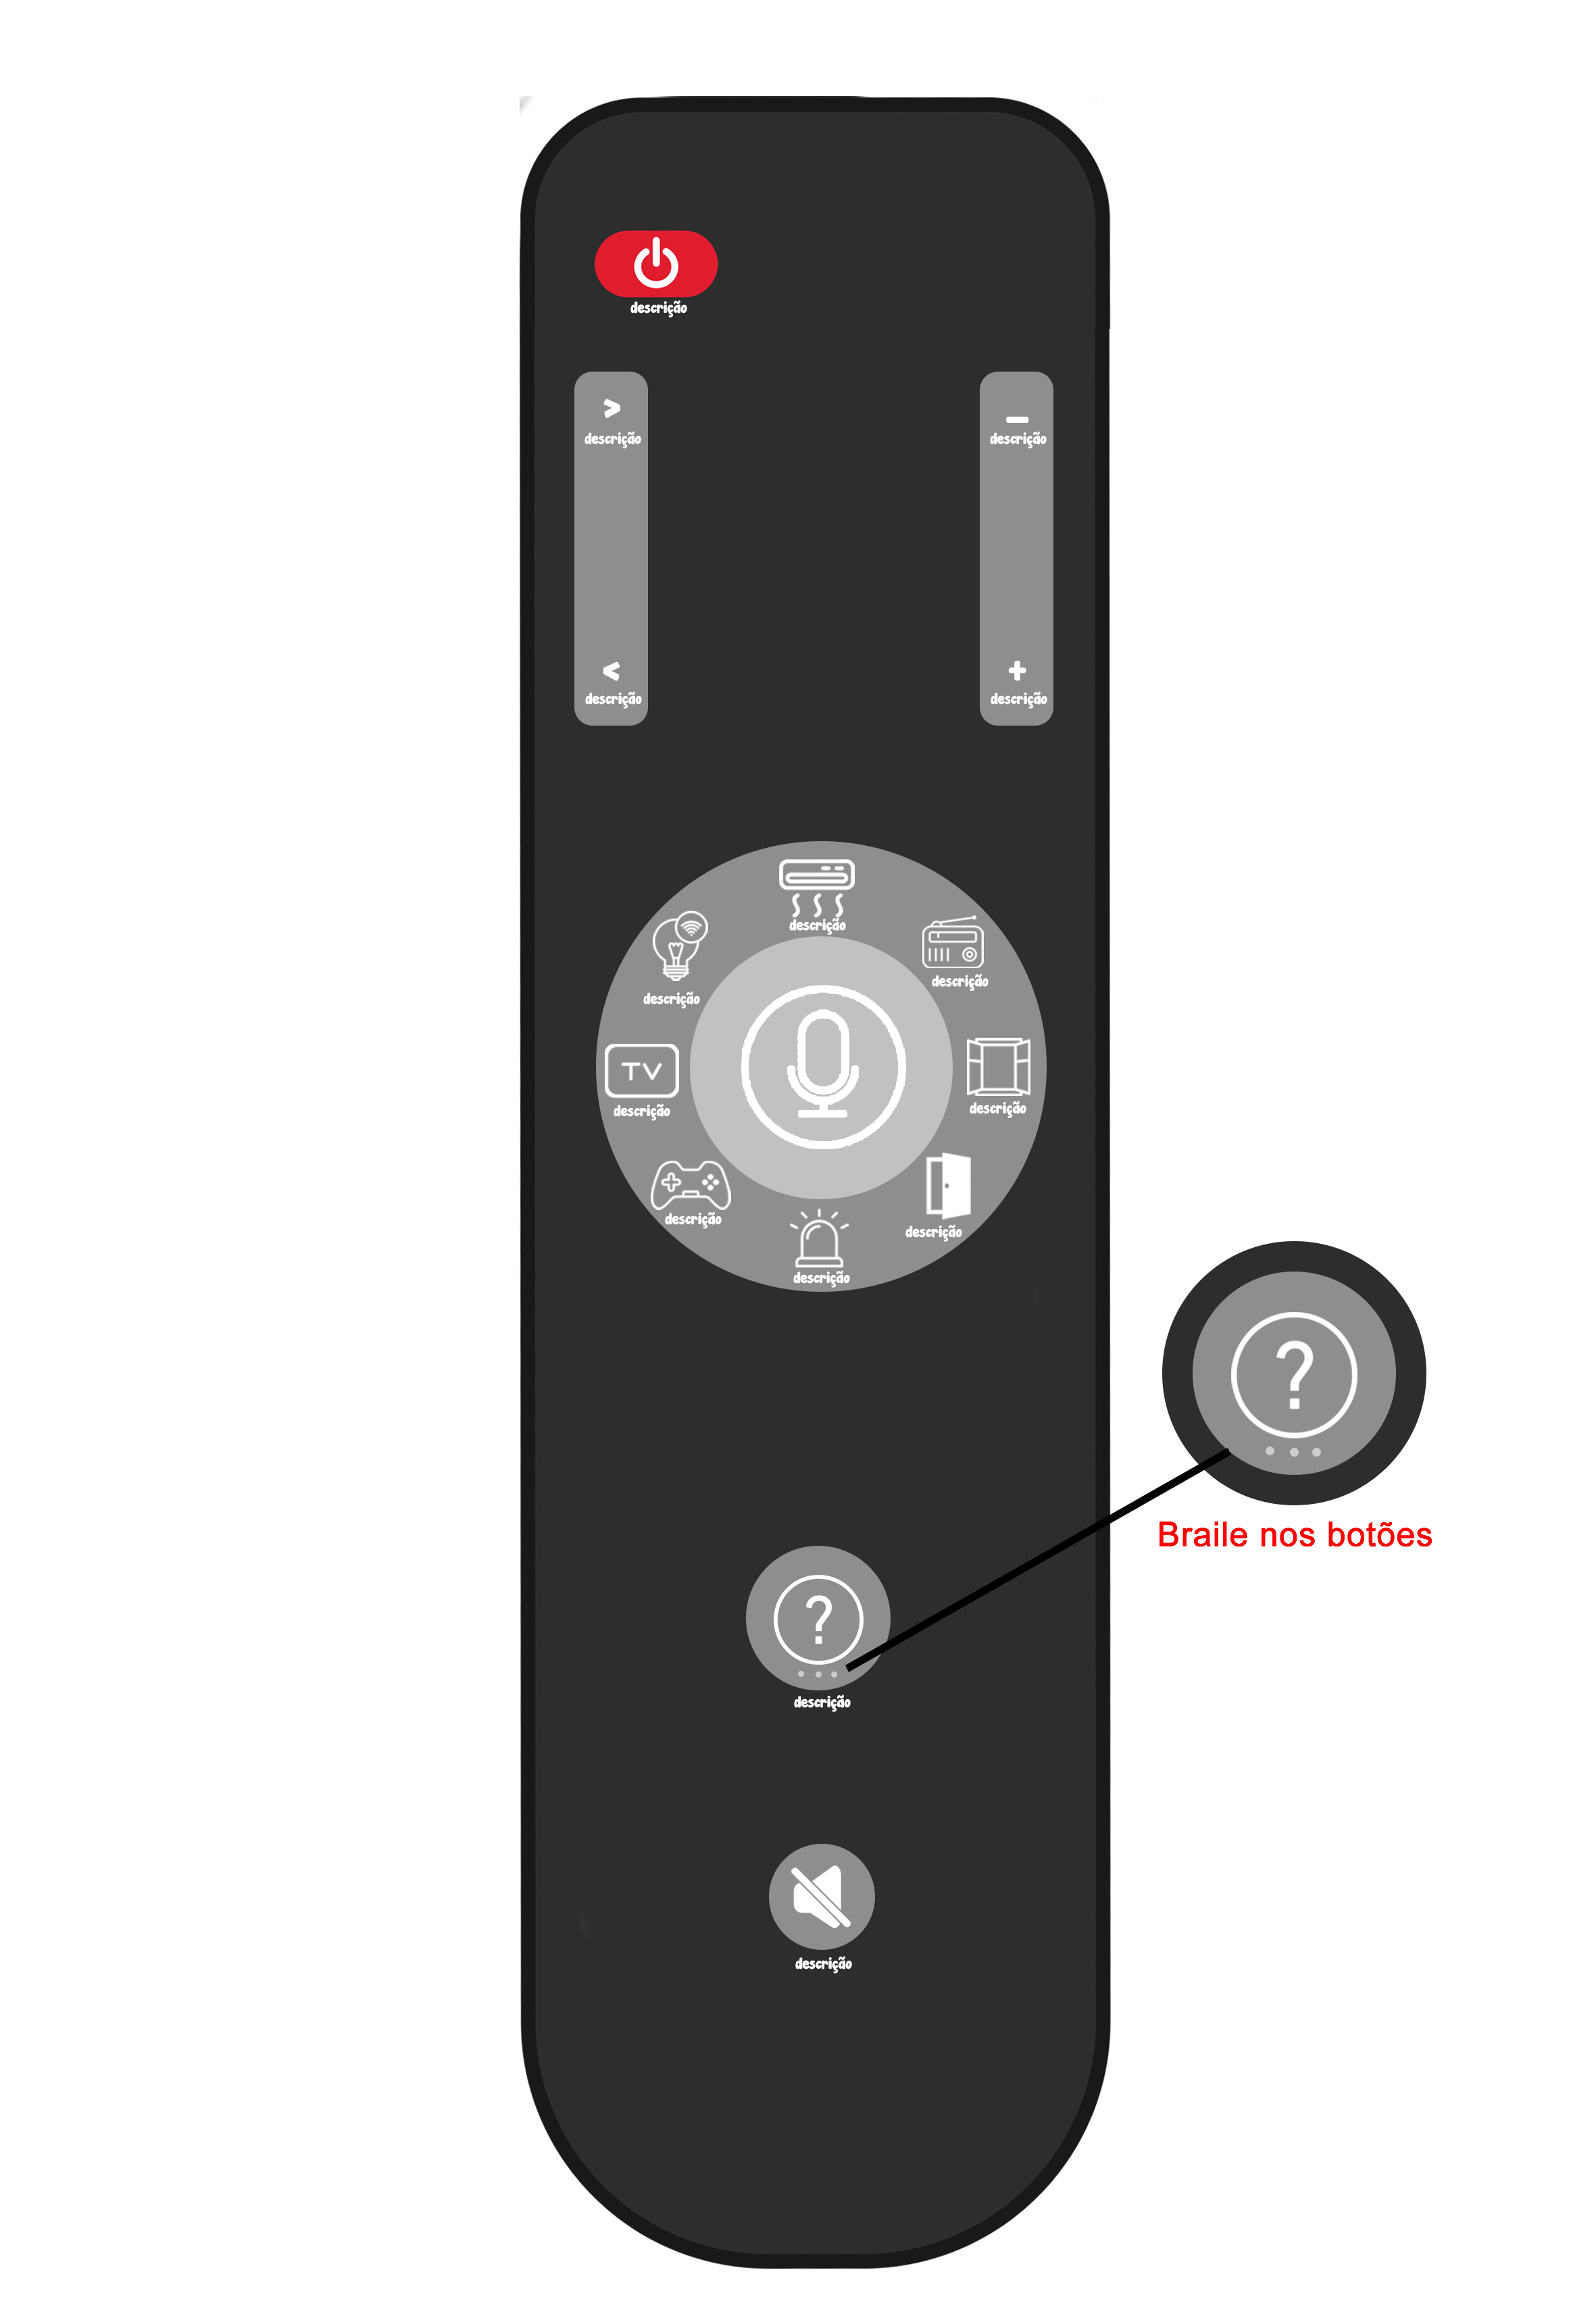
\includegraphics[width=14cm]{controle}
	\caption{Controle}
	\label{fig:controle}
\end{figure}

\section{Avaliação da interface}
\begin{itemize}
	\item \textbf{Visibilidade do status
		do sistema}: É possível visualizar pela alteração de cores quando é
			clicado sobre o botão.  No caso o verde a operação foi realizada com
			sucesso, o vermelho, houve uma possível falha e piscando é que a operação
			está sendo executada naquele momento.
	\item \textbf{Compatibilidade entre o sistema e o mundo real}: Os ícones que
		representam as funcionalidades dentro da interface do controle foram
		escolhidos de forma a facilitar a compreensão das funções, pois exibem
		figuras do cotidiano do usuário.
	\item \textbf{Controle e liberdade para o usuário}: O controle fornece
		liberdade ao usuário já que o mesmo pode interromper uma ação rapidamente
		clicando novamente no botão.
	\item \textbf{Consistência e padronização}: Na consistência e padronização do
		controle, o mesmo possui ícones dos quais representam objetos do dia a dia,
		como pode ser visto na imagem acima.
	\item \textbf{Prevenção de erros}: Para cada botão acionado o controle falará
		o nome da ação, para que usuário cegos não estejam conscientes em estar
		apertando um botão, sendo na verdade, que estão apertando outro botão
		totalmente diferente.
	\item \textbf{Reconhecimento ao invés de memorização}: Além dos ícones o
		controle organiza as funcionalidades que estão presentes no círculo central
		em ordem alfabética.
	\item \textbf{Eficiência e flexibilidade de uso}: Com adição de ícones e
		botões fica fácil do usuário mais leigo compreender a utilidade e
		funcionalidades do controle.
	\item \textbf{Estética e Design minimalista}: O layout do controle foi
		desenvolvido já pensando nos controles que existiam para não dificultar
		quanto a associação do equipamento e manter um estilo minimalista.
	\item \textbf{\sout{Ajude os usuários a reconhecerem, diagnosticarem e
		recuperarem-se de erros}}:
	\item \textbf{Ajuda e documentação}: O controle vem com um manual de
		instrução o qual também pode ser consultado pela internet.
\end{itemize}

\end{document}
